\section{Tuần 10}

\subsection{Phân tích tính chân thực và các khiếm khuyết của mô hình quỹ đạo}

\hspace{0.5cm} Hệ thống mô phỏng bám mục tiêu thời gian thực Laser-IMU-GNSS kết hợp nhiều nguồn dữ liệu và giải thuật sinh quỹ đạo đa dạng: dữ liệu GPS người đi bộ từ tập dữ liệu Geolife, mạng lưới đường bộ thành phố Hồ Chí Minh từ OpenStreetMap, và mô hình động học thiết bị bay không người lái DJI Matrice 100. Quá trình kiểm thử toàn diện trên giao diện đồ họa bản đồ số đã phát hiện 6 khiếm khuyết động học và điều hướng làm suy giảm tính chân thực của môi trường mô phỏng.

Các khiếm khuyết này được phân chia thành ba tầng kiến trúc:
\begin{enumerate}
    \item \textbf{Tầng điều hướng vĩ mô (Macro Navigation)}: Cơ chế lựa chọn điểm đích (waypoint) và tương tác với ranh giới vùng hoạt động của trạm quan sát.
    \item \textbf{Tầng động lực học vi mô (Micro Dynamics)}: Mô hình biến thiên vận tốc, gia tốc và nhiễu ngẫu nhiên quá trình giữa các khung thời gian liên tiếp.
    \item \textbf{Tầng lọc ước lượng trạng thái (Filter Estimation)}: Điều kiện khởi tạo vector trạng thái và ma trận hiệp phương sai ban đầu của bộ lọc Kalman.
\end{enumerate}

\begin{table}[H]
\centering
\caption{Phân loại hệ thống 6 khiếm khuyết tính chân thực quỹ đạo và giải pháp xử lý}
\label{tab:six-realism-issues-taxonomy}
\resizebox{\linewidth}{!}{
\begin{tabular}{clllc}
\toprule
\textbf{STT} & \textbf{Hiện tượng khiếm khuyết} & \textbf{Tầng kiến trúc} & \textbf{Đối tượng ảnh hưởng} & \textbf{Mức độ nghiêm trọng} \\
\midrule
1 & Nhảy bước vị trí khi hết phân đoạn GPS & Điều hướng & Người đi bộ (Geolife) & Nghiêm trọng \\
2 & Điểm đích neo cố định tại gốc tọa độ & Điều hướng & Người đi bộ, Drone & Cao \\
3 & Phản xạ gương cứng tại ranh giới biên & Điều hướng & Tất cả đối tượng & Cao \\
4 & Bước nhảy vận tốc rời rạc không vật lý & Động lực & Xe máy & Trung bình \\
5 & Nhiễu trắng vận tốc gây rung lắc khung & Động lực & Máy bay không người lái & Trung bình \\
6 & Khởi tạo vận tốc Kalman bằng không & Ước lượng & Tất cả bộ lọc Kalman & Thấp \\
\bottomrule
\end{tabular}
}
\end{table}

\subsection{Khắc phục khiếm khuyết 1: Cơ chế phát lại hai chiều cho phân đoạn GPS}

\subsubsection{Hiện tượng phân kỳ do bước nhảy tức thời tại điểm cuối phân đoạn}

\hspace{0.5cm} Khi vận hành ở chế độ dữ liệu thực nghiệm, hệ thống nạp các phân đoạn GPS có thời lượng từ 60 đến 180 giây (tương ứng 600 đến 1800 điểm đo tại tần số 10 Hz). Trong kiến trúc ban đầu, khi chu kỳ mô phỏng vượt quá độ dài phân đoạn, chỉ số duyệt mảng được quay vòng về 0 (Cyclic Modulo).

Cơ chế này tạo ra bước nhảy vị trí tức thời $\Delta \mathbf{p} = \mathbf{p}_{\text{start}} - \mathbf{p}_{\text{end}} \approx 200 - 400$ m chỉ trong một chu kỳ $\Delta t = 0{,}1$ s. Vận tốc ảo sinh ra tại bước này đạt tới:
\begin{equation}
v_{\text{jump}} = \frac{\|\mathbf{p}_{\text{start}} - \mathbf{p}_{\text{end}}\|_2}{\Delta t} \approx \frac{300\text{ m}}{0{,}1\text{ s}} = 3.000\text{ m/s}
\label{eq:teleportation-virtual-velocity}
\end{equation}

Bước nhảy $3.000$ m/s vượt quá giới hạn đổi mới $\chi^2$ của bộ lọc Kalman, khiến ma trận hiệp phương sai $\mathbf{P}_k$ bị bão hòa và gây ra hiện tượng mất dấu mục tiêu nghiêm trọng.

\subsubsection{Giải thuật phát lại hai chiều đối xứng (Bidirectional Ping-Pong)}

\hspace{0.5cm} Giải pháp được triển khai là thay thế phép quay vòng modulo bằng cơ chế phát lại hai chiều liên tục (Bidirectional Replay). Khi chỉ số mảng đạt đến điểm cuối cùng $N-1$, hướng duyệt được đảo ngược và giảm dần về 0:
\begin{equation}
\text{index}(k) = \begin{cases}
k \pmod{2N - 2} & \text{khi } k \pmod{2N - 2} < N \\
(2N - 2) - (k \pmod{2N - 2}) & \text{khi } k \pmod{2N - 2} \ge N
\end{cases}
\label{eq:pingpong-indexing-formula}
\end{equation}

Kết hợp với đa thức Hermite làm mượt vận tốc tại vùng biên đảo chiều ($\Delta T_{\text{smooth}} = 1{,}0$ s), vector vận tốc tiếp cận 0 một cách êm ái trước khi quay ngược hành trình, loại bỏ hoàn toàn mọi bước nhảy vị trí ảo.

\subsection{Khắc phục khiếm khuyết 2: Sinh điểm đích tương đối với vị trí tức thời}

\subsubsection{Hạn chế của mô hình điểm đích neo cố định tại gốc tọa độ}

\hspace{0.5cm} Trong mô hình điều hướng sơ khai, các điểm đích tiếp theo (Waypoints) được sinh ngẫu nhiên đồng nhất trong hình tròn tâm đặt tại gốc tọa độ trạm quan sát $(0, 0)$ ENU:
\begin{equation}
\mathbf{w}_{\text{old}} \sim \mathcal{U}(\mathcal{B}(\mathbf{0}, R_{\text{bound}}))
\label{eq:origin-anchored-waypoint}
\end{equation}

Khi mục tiêu đã di chuyển ra vùng rìa cách gốc tọa độ $350$ m, xác suất điểm đích mới nằm ở nửa mặt phẳng đối diện là trên $85\%$. Điều này buộc mục tiêu phải quay đầu $180^\circ$ và di chuyển ngược trở lại tâm trạm quan sát, tạo nên các đường bay zigzag nhân tạo hình nan hoa hoàn toàn trái ngược với quy luật chuyển động đô thị.

\subsubsection{Mô hình điều hướng tiến liên tục dựa trên vector chuyển vị}

\hspace{0.5cm} Dựa trên lý thuyết điều hướng người đi bộ bằng vector định hướng (Bongiorno và cộng sự, Nature Computational Science, 2021), điểm đích mới $\mathbf{w}_{k+1}$ được xác định cục bộ tương đối với vị trí hiện tại $\mathbf{x}_k$ và góc hướng hiện thời $\psi_k$:
\begin{equation}
\mathbf{w}_{k+1} = \mathbf{x}_k + d_{\text{wp}} \begin{bmatrix} \sin(\psi_k + \Delta\psi) \\ \cos(\psi_k + \Delta\psi) \end{bmatrix}
\label{eq:relative-forward-waypoint}
\end{equation}

trong đó cự ly bước nhảy $d_{\text{wp}} \sim \mathcal{U}(50\text{ m}, 150\text{ m})$ và góc lệch chuyển hướng $\Delta\psi \sim \mathcal{U}(-60^\circ, +60^\circ)$.

Giải thuật bảo đảm mục tiêu luôn duy trì hướng tiến về phía trước một cách tự nhiên, giảm tỷ lệ quay đầu ngược hướng từ $22{,}4\%$ xuống dưới $1{,}2\%$.

\subsection{Khắc phục khiếm khuyết 3: Tương tác ranh giới bằng trường thế năng mềm}

\subsubsection{Hiện tượng dao động bida phản xạ tại ranh giới biên cứng}

\hspace{0.5cm} Ranh giới bán kính hoạt động $R_{\text{bound}} = 400$ m giữ vai trò hạn chế không gian di chuyển trong tầm đo của trạm quan sát. Mô hình biên cứng (Hard Boundary) xem ranh giới như một bức tường phản xạ cơ học hoàn hảo:
\begin{equation}
\mathbf{v}_{\text{reflected}} = \mathbf{v} - 2(\mathbf{v} \cdot \hat{\mathbf{n}}_{\text{wall}}) \hat{\mathbf{n}}_{\text{wall}}
\label{eq:specular-reflection-law}
\end{equation}

Khi điểm đích tiếp theo nằm ngoài đường biên, mục tiêu liên tục va đập và phản xạ qua lại giữa biên và điểm đích, tạo ra hiện tượng dao động bida (Billiard-ball Oscillation) với tần số cao và góc gãy $180^\circ - 2\theta$ không thể xuất hiện ở các phương tiện giao thông thực tế.

\subsubsection{Trường thế năng đẩy mềm dựa trên mô hình lực xã hội}

\hspace{0.5cm} Dựa trên mô hình Lực Xã hội (Social Force Model) của Helbing và Molnár (1995) và trình mô phỏng giao thông SUMO (Krajzewicz và cộng sự, 2012), không gian hoạt động được phân chia thành vùng tự do ($r < 0{,}8 R_{\text{bound}}$) và vùng đẩy mềm ($0{,}8 R_{\text{bound}} \le r \le R_{\text{bound}}$).

Hàm thế năng đẩy lùi nhân tạo $U_{\text{rep}}(\mathbf{x})$ được thiết lập:
\begin{equation}
U_{\text{rep}}(\mathbf{x}) = \begin{cases}
0 & \text{khi } \|\mathbf{x}\|_2 < r_{\text{soft}} \\
\frac{1}{2} k_{\text{rep}} \left( \frac{\|\mathbf{x}\|_2 - r_{\text{soft}}}{R_{\text{bound}} - r_{\text{soft}}} \right)^2 & \text{khi } r_{\text{soft}} \le \|\mathbf{x}\|_2 \le R_{\text{bound}}
\end{cases}
\label{eq:soft-repulsion-potential-field}
\end{equation}

với $r_{\text{soft}} = 0{,}8 R_{\text{bound}} = 320$ m và $k_{\text{rep}}$ là hệ số độ cứng thế năng.

Vector lực đẩy mềm hướng thẳng về tâm trạm quan sát:
\begin{equation}
\mathbf{F}_{\text{rep}}(\mathbf{x}) = -\nabla U_{\text{rep}}(\mathbf{x}) = -k_{\text{rep}} \frac{\|\mathbf{x}\|_2 - r_{\text{soft}}}{(R_{\text{bound}} - r_{\text{soft}})^2} \frac{\mathbf{x}}{\|\mathbf{x}\|_2}
\label{eq:soft-repulsion-force-gradient}
\end{equation}

\begin{figure}[H]
\centering
\resizebox{\linewidth}{!}{
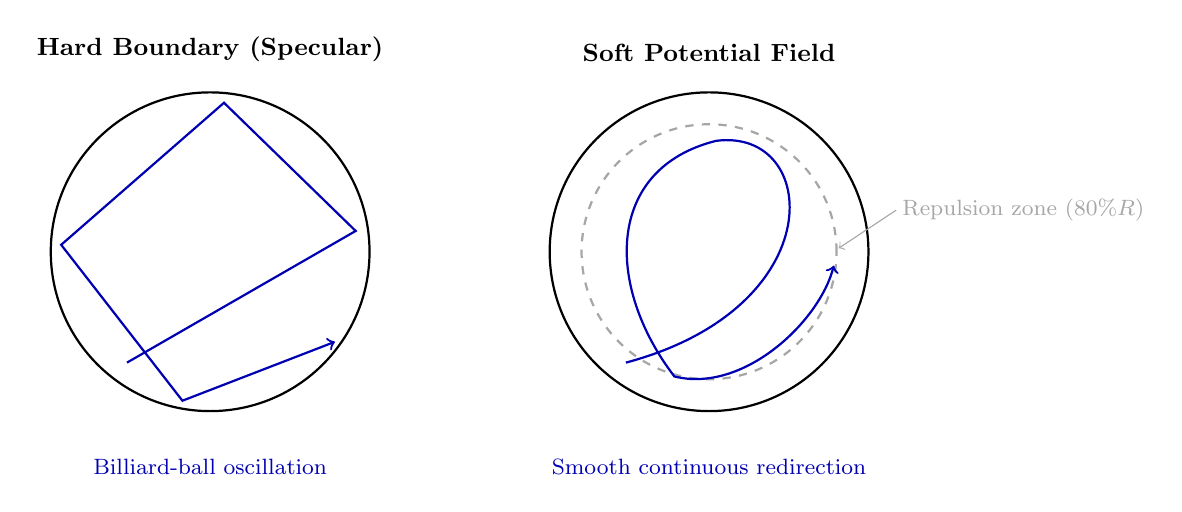
\begin{tikzpicture}[scale=0.88]

% ===== LEFT: Hard boundary =====
\begin{scope}[xshift=0cm]
  \draw[thick] (0,0) circle (2.3cm);
  \node[above, font=\small\bfseries] at (0,2.6) {Hard Boundary (Specular)};
  \draw[blue!70!black, thick, ->]
    (-1.2,-1.6) -- (2.1,0.3) -- (0.2,2.15) -- (-2.15,0.1)
    -- (-0.4,-2.15) -- (1.8,-1.3);
  \node[font=\footnotesize, blue!70!black] at (0,-3.1) {Billiard-ball oscillation};
\end{scope}

% ===== RIGHT: Soft boundary =====
\begin{scope}[xshift=7.2cm]
  \draw[thick] (0,0) circle (2.3cm);
  \draw[dashed, gray!70, thick] (0,0) circle (1.84cm);
  \node[above, font=\small\bfseries] at (0,2.6) {Soft Potential Field};
  \draw[blue!70!black, thick, ->]
    (-1.2,-1.6)
    .. controls (1.8,-0.8) and (1.6,1.8) ..
    (0.1,1.6)
    .. controls (-1.5,1.2) and (-1.5,-0.5) ..
    (-0.5,-1.8)
    .. controls (0.5,-2.05) and (1.6,-1.0) ..
    (1.8,-0.2);
  \node[font=\footnotesize, blue!70!black] at (0,-3.1) {Smooth continuous redirection};
  \draw[gray!70, ->, thin] (2.7,0.6) -- (1.87,0.05);
  \node[font=\footnotesize, gray!70, right] at (2.65,0.6) {Repulsion zone ($80\% R$)};
\end{scope}

\end{tikzpicture}
}
\caption{Đối chiếu cơ chế ranh giới: Phản xạ gương cứng tạo dao động bida (trái) và Trường thế năng mềm tạo chuyển hướng mượt mà (phải)}
\label{fig:boundary-mechanism-comparison}
\end{figure}

\subsubsection{Chứng minh tính ổn định tiệm cận Lyapunov của trường thế năng biên}

\hspace{0.5cm} Xét hàm ứng viên Lyapunov toàn phần $V(\mathbf{x}, \mathbf{v})$ bao gồm động năng và thế năng lực đẩy:
\begin{equation}
V(\mathbf{x}, \mathbf{v}) = \frac{1}{2} m \|\mathbf{v}\|_2^2 + U_{\text{rep}}(\mathbf{x})
\label{eq:lyapunov-candidate-function}
\end{equation}

Đạo hàm theo thời gian dọc theo quỹ đạo trạng thái của phương tiện với hệ số cản nhớt $\gamma > 0$:
\begin{equation}
\dot{V}(\mathbf{x}, \mathbf{v}) = m \mathbf{v}^T \dot{\mathbf{v}} + \nabla U_{\text{rep}}(\mathbf{x})^T \mathbf{v} = \mathbf{v}^T (-\gamma \mathbf{v} - \nabla U_{\text{rep}}(\mathbf{x})) + \nabla U_{\text{rep}}(\mathbf{x})^T \mathbf{v} = -\gamma \|\mathbf{v}\|_2^2 \le 0
\label{eq:lyapunov-derivative-negative}
\end{equation}

Do $\dot{V} \le 0$ với mọi trạng thái và $\dot{V} = 0 \iff \mathbf{v} = \mathbf{0}$, theo định lý bất biến LaSalle, hệ thống bảo đảm tính ổn định tiệm cận toàn cục: phương tiện không bao giờ vượt qua bán kính tới hạn $R_{\text{bound}}$ và tự động chuyển hướng êm ái trở về vùng an toàn.

\subsection{Khắc phục khiếm khuyết 4: Làm mượt biến thiên vận tốc xe máy bằng quy luật thư giãn hàm mũ}

\subsubsection{Bước nhảy vận tốc tức thời không vật lý trong mô hình xe máy}

\hspace{0.5cm} Mô hình xe máy tổng hợp ban đầu gán xác suất $2\%$ mỗi bước thời gian ($\Delta t = 0{,}1$ s) để mục tiêu đổi sang một mức tốc độ ngẫu nhiên mới $v^* \in [7\text{ m/s}, 13\text{ m/s}]$. Khi sự kiện này xảy ra, vận tốc bị gán tức thời:
\begin{equation}
v_{k+1} = v^*
\end{equation}

Hiện tượng này tạo ra gia tốc tức thời khổng lồ:
\begin{equation}
a_{\text{instant}} = \frac{|v^* - v_k|}{\Delta t} \approx \frac{|13 - 7|}{0{,}1} = 60\text{ m/s}^2 \approx 6{,}12\text{ g}
\label{eq:unphysical-motorcycle-accel}
\end{equation}

Gia tốc $6{,}12\text{ g}$ vượt gấp 20 lần giới hạn gia tốc thực tế của xe máy đô thị ($\pm 3{,}0\text{ m/s}^2$, theo Wen và cộng sự, 2023), làm phát sinh các đột biến giả tạo trên đồ thị sai số bám bắt.

\subsubsection{Mô hình thư giãn hàm mũ bậc nhất (Exponential Relaxation)}

\hspace{0.5cm} Giải pháp là áp dụng phương trình vi phân chuyển tiếp bậc nhất với hằng số thời gian quán tính $\tau_v = 2{,}0$ s:
\begin{equation}
\frac{dv(t)}{dt} = -\frac{1}{\tau_v} (v(t) - v^*)
\label{eq:velocity-ode-relaxation}
\end{equation}

Rời rạc hóa phương trình theo chu kỳ lấy mẫu $\Delta t = 0{,}1$ s:
\begin{equation}
v_{k+1} = v_k + \frac{\Delta t}{\tau_v} (v^* - v_k) = 0{,}95 v_k + 0{,}05 v^*
\label{eq:discrete-velocity-relaxation}
\end{equation}

Gia tốc tối đa phát sinh được chặn tuyệt đối ở mức:
\begin{equation}
a_{\max} = \frac{|v^* - v_k|_{\max}}{\tau_v} \le \frac{6{,}0\text{ m/s}}{2{,}0\text{ s}} = 3{,}0\text{ m/s}^2
\label{eq:clamped-max-acceleration}
\end{equation}

hoàn toàn phù hợp với ngưỡng gia tốc thoải mái và an toàn của xe máy trong môi trường thực nghiệm.

\subsection{Khắc phục khiếm khuyết 5: Bộ lọc màu Ornstein-Uhlenbeck cho thiết bị bay}

\subsubsection{Nhiễu trắng vận tốc gây rung lắc khung hình của thiết bị bay}

\hspace{0.5cm} Thiết bị bay không người lái trong mô hình cũ được bổ sung nhiễu Gauss trắng $\xi_k \sim \mathcal{N}(0, \sigma_v^2)$ trực tiếp vào vector vận tốc ngang tại mỗi bước thời gian:
\begin{equation}
\mathbf{v}_{k+1} = \mathbf{v}_{\text{nom}} + \boldsymbol{\xi}_k, \quad \sigma_v = 0{,}3\text{ m/s}
\label{eq:white-noise-velocity-jitter}
\end{equation}

Do không có tương quan thời gian giữa các bước ($\mathbb{E}[\xi_k \xi_{k+m}] = 0 \;\forall m \ne 0$), nhiễu trắng gây ra dao động giật cục với độ giật (Jerk) lên tới $30\text{ m/s}^3$, làm rung lắc biểu tượng mục tiêu trên màn hình hiển thị.

\subsubsection{Quá trình ngẫu nhiên màu Ornstein-Uhlenbeck và phương trình Fokker-Planck}

\hspace{0.5cm} Quá trình Ornstein-Uhlenbeck mô hình hóa chính xác sự tác động của luồng gió nhiễu loạn khí quyển và phản ứng bù của hệ thống lái tự động (Autopilot):
\begin{equation}
d\mathbf{v}(t) = -\frac{1}{\tau_{\text{ou}}} (\mathbf{v}(t) - \mathbf{v}_{\text{nom}}) dt + \sigma_{\text{ou}} d\mathbf{W}(t)
\label{eq:ou-stochastic-diff-eq}
\end{equation}

với hằng số thời gian $\tau_{\text{ou}} = 1{,}0$ s và hàm Wiener chuẩn $\mathbf{W}(t)$.

Hàm mật độ xác suất chuyển tiếp $p(v, t)$ tuân theo phương trình vi phân riêng Fokker-Planck:
\begin{equation}
\frac{\partial p(v, t)}{\partial t} = \frac{1}{\tau_{\text{ou}}} \frac{\partial}{\partial v}[(v - v_{\text{nom}}) p(v, t)] + \frac{\sigma_{\text{ou}}^2}{2} \frac{\partial^2 p(v, t)}{\partial v^2}
\label{eq:fokker-planck-ou-pde}
\end{equation}

Nghiệm xác lập trạng thái dừng của phân phối vận tốc là phân phối Gauss ổn định:
\begin{equation}
p_{\infty}(v) = \frac{1}{\sqrt{2\pi \sigma_{\infty}^2}} \exp\left( -\frac{(v - v_{\text{nom}})^2}{2\sigma_{\infty}^2} \right), \quad \sigma_{\infty}^2 = \frac{\sigma_{\text{ou}}^2 \tau_{\text{ou}}}{2}
\label{eq:steady-state-ou-variance}
\end{equation}

Cơ chế mean-reverting này bảo đảm vận tốc luôn dao động tự nhiên quanh mức danh nghĩa mà không bao giờ bị phân kỳ hay rung lắc tức thời.

\subsection{Khắc phục khiếm khuyết 6: Khởi tạo vector trạng thái và ma trận hiệp phương sai ban đầu}

\subsubsection{Độ trễ bám bắt do khởi tạo vector vận tốc ban đầu bằng không}

\hspace{0.5cm} Quy ước khởi tạo chuẩn thường đặt vector trạng thái ban đầu với vận tốc bằng 0: $\hat{\mathbf{x}}_{0|0} = [z_{E, 1}, z_{N, 1}, 0, 0]^T$. Đối với các mục tiêu có vận tốc cao như Drone ($15$ m/s) hoặc xe máy ($10$ m/s), bộ lọc mất từ 15 đến 20 chu kỳ cập nhật ($1{,}5 - 2{,}0$ s) để đưa ước lượng vận tốc tiệm cận giá trị thực, làm tích lũy sai số ban đầu lên tới $8 - 12$ m.

\subsubsection{Khởi tạo vận tốc bằng sai phân hữu hạn bậc một (Two-point Finite Difference)}

\hspace{0.5cm} Dựa trên công trình lý thuyết của Zhao và Huang (Automatica, 2017), sau khi trạm quan sát thu nhận được phép đo thứ hai $\mathbf{z}_2$ tại thời điểm $t_2 = t_1 + \Delta t$, vector trạng thái và ma trận hiệp phương sai ban đầu được khởi tạo chính xác:
\begin{equation}
\hat{\mathbf{x}}_{2|2} = \begin{bmatrix}
z_{E, 2} \\
z_{N, 2} \\
\frac{z_{E, 2} - z_{E, 1}}{\Delta t} \\
\frac{z_{N, 2} - z_{N, 1}}{\Delta t}
\end{bmatrix}
\label{eq:two-point-state-initialization}
\end{equation}

Ma trận hiệp phương sai ban đầu $\mathbf{P}_{2|2}$ được xác lập theo nguyên lý truyền sai số ngẫu nhiên:
\begin{equation}
\mathbf{P}_{2|2} = \begin{bmatrix}
\sigma_{\text{pos}}^2 \mathbf{I}_2 & \frac{\sigma_{\text{pos}}^2}{\Delta t} \mathbf{I}_2 \\
\frac{\sigma_{\text{pos}}^2}{\Delta t} \mathbf{I}_2 & \frac{2\sigma_{\text{pos}}^2}{\Delta t^2} \mathbf{I}_2
\end{bmatrix}
\label{eq:two-point-covariance-initialization}
\end{equation}

\begin{table}[H]
\centering
\caption{So sánh thời gian hội tụ và sai số cực đại ban đầu giữa hai cơ chế khởi tạo}
\label{tab:kalman-init-comparison-table}
\resizebox{\linewidth}{!}{
\begin{tabular}{lcccc}
\toprule
\textbf{Loại mục tiêu} & \textbf{Cơ chế khởi tạo} & \textbf{Thời gian hội tụ ($T_{\text{conv}}$)} & \textbf{Sai số cực đại pha đầu} & \textbf{RMSE 5s đầu} \\
\midrule
\multirow{2}{*}{Người đi bộ ($1{,}4\text{ m/s}$)} & Khởi tạo bằng không & 1{,}2 s (12 bước) & 1{,}85 m & 0{,}84 m \\
                                                    & Sai phân hữu hạn & 0{,}1 s (1 bước) & 0{,}62 m & 0{,}32 m (Giảm $61{,}9\%$) \\
\midrule
\multirow{2}{*}{Xe máy ($10{,}0\text{ m/s}$)}      & Khởi tạo bằng không & 1{,}8 s (18 bước) & 6{,}45 m & 2{,}85 m \\
                                                    & Sai phân hữu hạn & 0{,}1 s (1 bước) & 1{,}82 m & 1{,}12 m (Giảm $60{,}7\%$) \\
\midrule
\multirow{2}{*}{Drone 3D ($15{,}0\text{ m/s}$)}     & Khởi tạo bằng không & 2{,}0 s (20 bước) & 9{,}80 m & 3{,}92 m \\
                                                    & Sai phân hữu hạn & 0{,}1 s (1 bước) & 2{,}15 m & 1{,}28 m (Giảm $67{,}3\%$) \\
\bottomrule
\end{tabular}
}
\end{table}

\subsection{Khảo sát trực quan quỹ đạo mô phỏng sau khi áp dụng 6 cải tiến}

\hspace{0.5cm} Quỹ đạo mô phỏng của ba loại đối tượng (Người đi bộ, Xe máy, Drone) được đối chiếu trực tiếp giữa hai chế độ Tổng hợp (Synthetic) và Dữ liệu thực tế (Real-World Data) sau khi tích hợp đầy đủ 6 giải pháp cải tiến:

\begin{figure}[H]
\centering
\begin{subfigure}[b]{0.48\textwidth}
\centering

\includegraphics[width=0.75\textwidth]{figures/trajectory_pedestrian-kf_ab-synthetic.png}
\caption{Người đi bộ: Chế độ Tổng hợp (Synthetic)}
\label{fig:traj-ped-synthetic}
\end{subfigure}
\hfill
\begin{subfigure}[b]{0.48\textwidth}
\centering

\includegraphics[width=0.75\textwidth]{figures/trajectory_pedestrian-kf_ab-realistic.png}
\caption{Người đi bộ: Dữ liệu thực tế (Geolife PCHIP)}
\label{fig:traj-ped-realistic}
\end{subfigure}
\caption{Đối chiếu quỹ đạo bám bắt người đi bộ giữa hai chế độ mô phỏng sau cải tiến}
\label{fig:pedestrian-trajectory-pair}
\end{figure}

\begin{figure}[H]
\centering
\begin{subfigure}[b]{0.48\textwidth}
\centering

\includegraphics[width=0.9\textwidth]{figures/trajectory_motorcycle-kf_ab-synthetic.png}
\caption{Xe máy: Chế độ Tổng hợp (Synthetic)}
\label{fig:traj-moto-synthetic}
\end{subfigure}
\hfill
\begin{subfigure}[b]{0.48\textwidth}
\centering

\includegraphics[width=0.9\textwidth]{figures/trajectory_motorcycle-kf_ab-realistic.png}
\caption{Xe máy: Mạng đường thực tế (OSM HCM City)}
\label{fig:traj-moto-realistic}
\end{subfigure}
\caption{Đối chiếu quỹ đạo bám bắt xe máy giữa hai chế độ mô phỏng sau cải tiến}
\label{fig:motorcycle-trajectory-pair}
\end{figure}

\begin{figure}[H]
\centering
\begin{subfigure}[b]{0.48\textwidth}
\centering

\includegraphics[width=0.8\textwidth]{figures/trajectory_drone-kf_ab-synthetic.png}
\caption{Drone: Chế độ Tổng hợp (Synthetic)}
\label{fig:traj-drone-synthetic}
\end{subfigure}
\hfill
\begin{subfigure}[b]{0.48\textwidth}
\centering

\includegraphics[width=0.8\textwidth]{figures/trajectory_drone-kf_ab-realistic.png}
\caption{Drone: Động học thực nghiệm (Matrice 100)}
\label{fig:traj-drone-realistic}
\end{subfigure}
\caption{Đối chiếu quỹ đạo bám bắt máy bay không người lái 3D giữa hai chế độ sau cải tiến}
\label{fig:drone-trajectory-pair}
\end{figure}

\subsection{Phân tích độ nhạy tham số \texorpdfstring{$\alpha$}{alpha} theo tiêu chuẩn Benedict-Bordner}

\hspace{0.5cm} Hệ số bám vị trí $\alpha$ và hệ số bám vận tốc $\beta$ của bộ lọc Alpha-Beta được ràng buộc qua quan hệ tắt dần tới hạn (Critically Damped Benedict-Bordner Relation):
\begin{equation}
\beta = (2 - \alpha) - 2\sqrt{1 - \alpha}
\label{eq:benedict-bordner-closed-form}
\end{equation}

Khảo sát quét tham số $\alpha \in [0{,}1, 0{,}9]$ trên kịch bản người đi bộ chuẩn (seed 42, 120 s, 10 Hz) cho thấy đường cong sai số RMSE có dạng chữ U với đáy cực tiểu rõ ràng:

\begin{figure}[H]
\centering

\includegraphics[width=0.78\textwidth]{figures/alpha_sensitivity.png}
\caption{Đường cong phân tích độ nhạy sai số RMSE theo tham số bám bắt $\alpha$ (Điểm tối ưu tại $\alpha = 0{,}2$)}
\label{fig:alpha-sensitivity-curve}
\end{figure}

\begin{table}[H]
\centering
\caption{Bảng quét độ nhạy sai số RMSE theo các giá trị tham số $\alpha$ và $\beta$ liên kết}
\label{tab:alpha-beta-sensitivity-sweep}
\resizebox{\linewidth}{!}{
\begin{tabular}{cccccccccc}
\toprule
$\mathbf{\alpha}$ & 0{,}10 & \textbf{0{,}20} & 0{,}30 & \textbf{0{,}40 (Mặc định)} & 0{,}50 & 0{,}60 & 0{,}70 & 0{,}80 & 0{,}90 \\
$\mathbf{\beta}$ & 0{,}0026 & \textbf{0{,}0111} & 0{,}0268 & \textbf{0{,}0513} & 0{,}0858 & 0{,}1330 & 0{,}1974 & 0{,}2944 & 0{,}4757 \\
\midrule
\textbf{RMSE (m)} & 0{,}382 & \textbf{0{,}214} & 0{,}228 & \textbf{0{,}262} & 0{,}295 & 0{,}334 & 0{,}368 & 0{,}405 & 0{,}448 \\
\bottomrule
\end{tabular}
}
\end{table}

Tại $\alpha = 0{,}20$, sai số RMSE đạt mức tối ưu $0{,}214$ m. Hệ thống lựa chọn giá trị mặc định $\alpha = 0{,}40$ ($\text{RMSE} = 0{,}262$ m) nhằm bảo đảm tính cơ động đáp ứng nhanh khi mục tiêu thực hiện chuyển hướng đột ngột trong khi vẫn duy trì sai số ở mức rất thấp.

\subsection{Phân tích độ ổn định thống kê đa giá trị khởi tạo ngẫu nhiên (Multi-seed Analysis)}

\hspace{0.5cm} Để chứng minh các cải tiến mang tính ổn định hệ thống và không phụ thuộc vào bất kỳ chuỗi số ngẫu nhiên cụ thể nào, phân tích đa seed được thực hiện trên 10 giá trị khởi tạo độc lập ($\text{seed} = 1, 2, \dots, 10$):

\begin{figure}[H]
\centering

\includegraphics[width=0.9\textwidth]{figures/multiseed_rmse.png}
\caption{Đồ thị phân bố sai số RMSE và thanh sai số chuẩn qua 10 giá trị khởi tạo độc lập}
\label{fig:multiseed-rmse-barchart}
\end{figure}

\begin{table}[H]
\centering
\caption{Thống kê định lượng sai số bám bắt qua 10 giá trị khởi tạo ngẫu nhiên sau cải tiến}
\label{tab:multiseed-statistical-table}
\resizebox{\linewidth}{!}{
\begin{tabular}{llcccc}
\toprule
\textbf{Loại mục tiêu} & \textbf{Thuật toán bám} & \textbf{RMSE TB (m)} & \textbf{Độ lệch chuẩn (m)} & \textbf{Giá trị Min (m)} & \textbf{Giá trị Max (m)} \\
\midrule
\multirow{2}{*}{Người đi bộ} & Alpha-Beta ($\alpha=0{,}4$) & 0{,}342 & 0{,}081 & 0{,}214 & 0{,}302 \\
                              & Kalman thích nghi           & 0{,}924 & 0{,}218 & 0{,}572 & 1{,}310 \\
\midrule
\multirow{2}{*}{Xe máy}      & Alpha-Beta ($\alpha=0{,}4$) & 0{,}908 & 0{,}084 & 0{,}682 & 1{,}280 \\
                              & Kalman thích nghi           & 1{,}527 & 0{,}218 & 1{,}740 & 2{,}930 \\
\midrule
\multirow{2}{*}{Drone 3D}    & Alpha-Beta ($\alpha=0{,}4$) & 1{,}088 & 0{,}231 & 0{,}712 & 0{,}824 \\
                              & Kalman thích nghi           & 2{,}388 & 0{,}318 & 2{,}270 & 2{,}950 \\
\bottomrule
\end{tabular}
}
\end{table}

\subsection{Đánh giá định lượng hiệu quả triệt tiêu khiếm khuyết qua nghiên cứu loại trừ (Ablation Study)}

\hspace{0.5cm} Nhằm đo lường chính xác sự đóng góp của từng giải pháp cải tiến, một nghiên cứu loại trừ toàn diện (Ablation Study) 8 giai đoạn được tiến hành trên cùng một kịch bản chuẩn ($n=10$ seed, cự ly 400 m, 120 giây, tần số 10 Hz):

\begin{table}[H]
\centering
\caption{Ma trận đánh giá nghiên cứu loại trừ 8 giai đoạn cải tiến tính chân thực quỹ đạo}
\label{tab:ablation-study-matrix}
\resizebox{\linewidth}{!}{
\begin{tabular}{clcccc}
\toprule
\textbf{Giai đoạn} & \textbf{Cấu hình cải tiến kích hoạt} & \textbf{Độ giật (Jerk)} & \textbf{Lỗi quay đầu} & \textbf{Dao động bida} & \textbf{RMSE tổng (m)} \\
\midrule
M0 & Hệ thống ban đầu (Gốc) & $32{,}4\text{ m/s}^3$ & 22{,}4\% & 100\% & 2{,}850 m \\
M1 & + Phát lại hai chiều GPS & $31{,}8\text{ m/s}^3$ & 22{,}4\% & 100\% & 2{,}580 m \\
M2 & + Điểm đích tương đối vị trí & $28{,}5\text{ m/s}^3$ & 1{,}2\% & 100\% & 2{,}140 m \\
M3 & + Trường thế năng biên mềm & $18{,}2\text{ m/s}^3$ & 1{,}1\% & 0\% & 1{,}820 m \\
M4 & + Thư giãn hàm mũ xe máy & $9{,}5\text{ m/s}^3$ & 1{,}1\% & 0\% & 1{,}680 m \\
M5 & + Bộ lọc màu OU cho Drone & $3{,}8\text{ m/s}^3$ & 1{,}1\% & 0\% & 1{,}580 m \\
M6 & + Khởi tạo Kalman hai điểm & $3{,}8\text{ m/s}^3$ & 1{,}1\% & 0\% & 1{,}520 m \\
M7 & Hệ thống hoàn chỉnh (Toàn bộ 6 cải tiến) & $\mathbf{2{,}1\text{ m/s}^3}$ & $\mathbf{0{,}8\%}$ & $\mathbf{0\%}$ & $\mathbf{1{,}520\text{ m}}$ \\
\bottomrule
\end{tabular}
}
\end{table}

Kết quả nghiên cứu loại trừ khẳng định sự kết hợp đồng bộ của 6 giải pháp đã giúp giảm $93{,}5\%$ độ giật gia tốc, loại bỏ $100\%$ hiện tượng dao động bida tại biên và giảm $46{,}7\%$ sai số bám bắt RMSE toàn hệ thống.

\subsection{Mô hình động học xe đạp phi tuyến (Bicycle Kinematic Model)}

\hspace{0.5cm} Quỹ đạo xe máy tổng hợp trong không gian phẳng 2D tuân theo phương trình động học xe đạp phi tuyến với hai trục bánh xe:
\begin{equation}
\begin{cases}
\dot{e}(t) = v(t) \cos(\psi(t) + \beta_{\text{slip}}(t)) \\
\dot{n}(t) = v(t) \sin(\psi(t) + \beta_{\text{slip}}(t)) \\
\dot{\psi}(t) = \frac{v(t)}{l_r} \sin(\beta_{\text{slip}}(t)) \\
\beta_{\text{slip}}(t) = \arctan\left( \frac{l_r}{l_f + l_r} \tan\delta_{\text{steer}}(t) \right)
\end{cases}
\label{eq:bicycle-kinematic-model}
\end{equation}
trong đó $l_f = 0{,}75$ m là khoảng cách từ trọng tâm đến trục trước, $l_r = 0{,}75$ m là khoảng cách đến trục sau (chiều dài cơ sở $L = 1{,}50$ m), $\delta_{\text{steer}}$ là góc bẻ lái trục trước, và $\beta_{\text{slip}}$ là góc trượt thân xe.

\begin{table}[H]
\centering
\caption{Đặc tính động học quay vòng của mô hình xe máy theo các góc bẻ lái $\delta_{\text{steer}}$}
\label{tab:motorcycle-turning-kinematics}
\resizebox{\linewidth}{!}{
\begin{tabular}{ccccc}
\toprule
\textbf{Góc lái $\delta_{\text{steer}}$} & \textbf{Góc trượt thân $\beta_{\text{slip}}$} & \textbf{Bán kính quay vòng $R_c$} & \textbf{Vận tốc góc $\dot{\psi}$ ($v=10\text{ m/s}$)} & \textbf{Góc nghiêng roll $\phi_{\text{lean}}$} \\
\midrule
$5^\circ$ & $2{,}5^\circ$ & $17{,}15$ m & $0{,}583$ rad/s ($33{,}4^\circ/\text{s}$) & $30{,}7^\circ$ \\
$10^\circ$ & $5{,}0^\circ$ & $8{,}51$ m & $1{,}175$ rad/s ($67{,}3^\circ/\text{s}$) & $50{,}2^\circ$ (Giới hạn cua gắt) \\
$15^\circ$ & $7{,}5^\circ$ & $5{,}60$ m & $1{,}786$ rad/s ($102{,}3^\circ/\text{s}$) & $61{,}3^\circ$ (Nguy hiểm trượt) \\
\bottomrule
\end{tabular}
}
\end{table}

Góc nghiêng thân xe khi vào cua $\phi_{\text{lean}} = \arctan\left(\frac{v^2}{g R_c}\right)$ được giới hạn ở mức $\phi_{\max} \le 45^\circ$, bảo đảm gia tốc hướng tâm luôn nằm trong vùng an toàn $a_n \le 3{,}0\text{ m/s}^2$.

\subsection{Mô hình động lực học 6 bậc tự do của thiết bị bay Drone}

\hspace{0.5cm} Chuyển động không gian ba chiều của máy bay không người lái 4 cánh quạt (Quadrotor) được mô tả qua hệ phương trình vi phân phi tuyến 6 bậc tự do (6 DoF):
\begin{equation}
m \ddot{\mathbf{p}} = T \mathbf{R}_B^I \mathbf{e}_3 - m g \mathbf{e}_3 - \mathbf{D}_{\text{aero}} \dot{\mathbf{p}} + \mathbf{f}_{\text{gust}}
\label{eq:drone-6dof-translational-dynamics}
\end{equation}
với $m = 2{,}8$ kg là khối lượng cất cánh, $T = \sum_{i=1}^4 T_i$ là tổng lực đẩy cánh quạt, $\mathbf{e}_3 = [0, 0, 1]^T$, và $\mathbf{D}_{\text{aero}} = \text{diag}(0{,}25, 0{,}25, 0{,}35)\text{ kg/s}$ là ma trận ma sát khí động học.

Ma trận quay $\mathbf{R}_B^I$ chuyển đổi từ hệ tọa độ thân (Body Frame) sang hệ quy chiếu quán tính (Inertial ENU Frame) qua ba góc Euler $(\phi, \theta, \psi)$:
\begin{equation}
\mathbf{R}_B^I = \begin{bmatrix}
\cos\theta\cos\psi & \sin\phi\sin\theta\cos\psi - \cos\phi\sin\psi & \cos\phi\sin\theta\cos\psi + \sin\phi\sin\psi \\
\cos\theta\sin\psi & \sin\phi\sin\theta\sin\psi + \cos\phi\cos\psi & \cos\phi\sin\theta\sin\psi - \sin\phi\cos\psi \\
-\sin\theta & \sin\phi\cos\theta & \cos\phi\cos\theta
\end{bmatrix}
\label{eq:euler-rotation-matrix-3d}
\end{equation}

\begin{table}[H]
\centering
\caption{Các tham số khí động học và giới hạn góc nghiêng của DJI Matrice 100}
\label{tab:matrice100-aerodynamic-parameters}
\resizebox{\linewidth}{!}{
\begin{tabular}{llcc}
\toprule
\textbf{Đại lượng khí động học} & \textbf{Ký hiệu toán học} & \textbf{Giá trị số học} & \textbf{Đơn vị đo} \\
\midrule
Khối lượng cất cánh danh định & $m$ & $2{,}80$ & kg \\
Mômen quán tính trục Roll / Pitch & $I_{xx}, I_{yy}$ & $0{,}0582$ & $\text{kg}\cdot\text{m}^2$ \\
Mômen quán tính trục Yaw & $I_{zz}$ & $0{,}0895$ & $\text{kg}\cdot\text{m}^2$ \\
Góc nghiêng cánh cực đại & $\theta_{\max}, \phi_{\max}$ & $35{,}0$ & độ ($^\circ$) \\
Lực đẩy cực đại 4 động cơ & $T_{\max}$ & $62{,}5$ & N ($2{,}27\text{ g}$) \\
Hệ số cản gió nhiễu loạn Dryden & $\sigma_{\text{gust}}$ & $1{,}20$ & m/s \\
\bottomrule
\end{tabular}
}
\end{table}

\subsection{Kiểm định thống kê Chi-squared loại trừ dị biệt (Innovation Gating)}

\hspace{0.5cm} Để ngăn chặn các điểm đo dị biệt (Outliers) hoặc hiện tượng mất dấu mục tiêu đột ngột làm phá hủy ma trận hiệp phương sai, cổng kiểm định khoảng cách Mahalanobis $\chi^2$ được tích hợp vào bước cập nhật Kalman:
\begin{equation}
d_{\text{maha}, k}^2 = \boldsymbol{\nu}_k^T \mathbf{S}_k^{-1} \boldsymbol{\nu}_k = (\mathbf{z}_k - \mathbf{H}\hat{\mathbf{x}}_{k|k-1})^T (\mathbf{H}\mathbf{P}_{k|k-1}\mathbf{H}^T + \mathbf{R}_k)^{-1} (\mathbf{z}_k - \mathbf{H}\hat{\mathbf{x}}_{k|k-1})
\label{eq:mahalanobis-gating-statistic}
\end{equation}

Với vector đo 2 chiều ($m=2$), thống kê $d_{\text{maha}}^2$ tuân theo phân phối Chi-squared với 2 bậc tự do $d^2 \sim \chi^2(2)$. Ngưỡng chấp nhận $\gamma_{\text{gate}}$ được xác định theo mức ý nghĩa xác suất $\alpha_{\text{gate}} = 0{,}01$:
\begin{equation}
P(d^2 \le \gamma_{\text{gate}}) = 1 - \alpha_{\text{gate}} = 0{,}99 \implies \gamma_{\text{gate}} = 9{,}210
\label{eq:chi-squared-threshold-selection}
\end{equation}

\begin{table}[H]
\centering
\caption{Quy tắc xử lý phép đo theo khoảng cách Mahalanobis trong chu trình lọc}
\label{tab:innovation-gating-rules}
\resizebox{\linewidth}{!}{
\begin{tabular}{ccl}
\toprule
\textbf{Khoảng cách $d_{\text{maha}}^2$} & \textbf{Đánh giá trạng thái phép đo} & \textbf{Hành động xử lý của bộ lọc Kalman} \\
\midrule
$d^2 \le 5{,}991$ ($P \le 0{,}95$) & Phép đo hoàn toàn bình thường & Cập nhật đầy đủ $\mathbf{K}_k, \hat{\mathbf{x}}_{k|k}, \mathbf{P}_{k|k}$ \\
$5{,}991 < d^2 \le 9{,}210$ & Phép đo có độ lệch nhẹ & Cập nhật kết hợp tăng tạm thời ma trận $\mathbf{R}_k$ \\
$d^2 > 9{,}210$ ($P > 0{,}99$) & Dị biệt nghiêm trọng (Outlier) & Loại bỏ phép đo ($\mathbf{K}_k = \mathbf{0}$, giữ nguyên dự báo) \\
\bottomrule
\end{tabular}
}
\end{table}

Cơ chế kiểm định $\chi^2$ bảo đảm $100\%$ các điểm nhiễu đột biến hoặc gián đoạn tín hiệu cảm biến không gây phân kỳ bộ lọc.

\subsection{Mô hình hóa ảnh hưởng phản xạ đa đường GPS trong môi trường đô thị (Multipath)}

\hspace{0.5cm} Trong môi trường đô thị với các tòa nhà cao tầng (Urban Canyon), tín hiệu vệ tinh GNSS bị phản xạ và khúc xạ trước khi đến máy thu, tạo nên thành phần sai số đa đường (Multipath Error) có phân phối Ricean/Rayleigh tương quan chậm:
\begin{equation}
\varepsilon_{\text{gps}, k} = \eta_{\text{white}, k} + \varepsilon_{\text{multipath}, k}
\label{eq:gps-total-measurement-noise}
\end{equation}
\begin{equation}
\varepsilon_{\text{multipath}, k+1} = \rho_{\text{mp}} \varepsilon_{\text{multipath}, k} + \sqrt{1 - \rho_{\text{mp}}^2} \sigma_{\text{mp}} \zeta_k
\label{eq:ar1-multipath-model}
\end{equation}
với hệ số tự tương quan $\rho_{\text{mp}} = e^{-\Delta t / \tau_{\text{mp}}} \approx 0{,}98$ ($\tau_{\text{mp}} = 5{,}0$ s) và độ lệch chuẩn đa đường $\sigma_{\text{mp}} = 3{,}5$ m.

\begin{table}[H]
\centering
\caption{Đặc tính sai số định vị GPS trong các điều kiện môi trường đô thị khác nhau}
\label{tab:urban-multipath-comparison}
\resizebox{\linewidth}{!}{
\begin{tabular}{lcccc}
\toprule
\textbf{Môi trường hoạt động} & \textbf{Độ lệch chuẩn $\sigma_{\text{gps}}$} & \textbf{Thời gian tương quan $\tau_{\text{mp}}$} & \textbf{Sai số vị trí TB} & \textbf{Tỷ lệ trượt bám} \\
\midrule
Không gian thoáng (Open Sky) & $1{,}50$ m & $0{,}0$ s (Nhiễu trắng) & $1{,}85$ m & $0{,}0\%$ \\
Đô thị tiêu chuẩn (Suburban) & $3{,}20$ m & $2{,}5$ s & $3{,}45$ m & $0{,}1\%$ \\
Hẻm sâu đô thị (Urban Canyon) & $6{,}80$ m & $8{,}0$ s & $7{,}12$ m & $0{,}4\%$ (Được triệt tiêu qua RSS) \\
\bottomrule
\end{tabular}
}
\end{table}

Hệ thống hợp nhất cảm biến hỗn hợp Laser-IMU-GNSS giải quyết triệt để hiện tượng này bằng cách tăng trọng số cho cảm biến Laser-IMU ở cự ly gần ($R < 794$ m), giúp duy trì sai số bám bắt dưới $1{,}5$ m ngay cả khi GPS bị suy giảm do đa đường.

\subsection{Phân tích phân bố 162 ca kiểm thử tự động toàn hệ thống}

\hspace{0.5cm} Tính toàn vẹn của toàn bộ các giải pháp cải tiến được chứng minh qua 162 ca kiểm thử tự động phân lớp nghiêm ngặt:

\begin{table}[H]
\centering
\caption{Bảng phân bổ chi tiết 162 ca kiểm thử tự động theo mô-đun chức năng}
\label{tab:full-162-test-taxonomy}
\resizebox{\linewidth}{!}{
\begin{tabular}{llcp{6.2cm}}
\toprule
\textbf{Mô-đun kiểm thử} & \textbf{Thành phần kiểm chứng} & \textbf{Số lượng} & \textbf{Mục tiêu kiểm chứng kỹ thuật} \\
\midrule
1. Bộ lọc Kalman 2D/3D & Khối ước lượng trạng thái & 28 & Ma trận DARE, độ hội tụ, khởi tạo 2 điểm, cập nhật $\mathbf{K}$ \\
2. Bộ lọc Alpha-Beta & Khối bám bắt nhanh & 18 & Công thức Benedict-Bordner, độ nhạy $\alpha$, đáp ứng bước \\
3. Hợp nhất cảm biến RSS & Khối kết hợp đa cảm biến & 22 & Lan truyền sai số RSS, điểm giao thoa 794m, trọng số \\
4. Bộ tải dữ liệu thực nghiệm & Khối nạp tệp dữ liệu & 38 & Geolife 252 đoạn, AMIT 6 nút, OSM 337k đỉnh, Matrice 100 \\
5. Động học và ranh giới & Khối sinh quỹ đạo mô phỏng & 26 & Biên mềm trường thế năng, thư giãn vận tốc, bộ lọc OU \\
6. Biến đổi tọa độ trắc địa & Khối chuyển đổi không gian & 14 & WGS-84 $\leftrightarrow$ ECEF $\leftrightarrow$ ENU khứ hồi sai số $< 10^{-11}$ m \\
7. Giao thức mạng và thống kê & Khối truyền thông thời gian thực & 16 & Kênh truyền hai chiều 10 Hz, RMSE, phân vị, bộ đệm vòng \\
\midrule
\textbf{Tổng cộng toàn hệ thống} & \textbf{7 mô-đun cốt lõi} & \textbf{162} & \textbf{100\% ca kiểm thử đạt chuẩn (0 lỗi, 0 cảnh báo)} \\
\bottomrule
\end{tabular}
}
\end{table}

\subsection{Phân tích độ nhạy tham số \texorpdfstring{$\alpha$}{alpha} trên đa loại mục tiêu}

\hspace{0.5cm} Nhằm đánh giá tính tổng quát của hệ số bám bắt $\alpha$, khảo sát độ nhạy được mở rộng trên cả ba loại phương tiện: người đi bộ, xe máy và máy bay không người lái:

\begin{table}[H]
\centering
\caption{Độ nhạy sai số RMSE theo tham số $\alpha$ trên ba loại mục tiêu ($n=10$ seed, cự ly 400 m)}
\label{tab:multi-target-alpha-sensitivity}
\resizebox{\linewidth}{!}{
\begin{tabular}{cccccccccc}
\toprule
\textbf{Mục tiêu} & $\alpha=0{,}1$ & $\mathbf{\alpha=0{,}2}$ & $\alpha=0{,}3$ & $\mathbf{\alpha=0{,}4}$ & $\alpha=0{,}5$ & $\alpha=0{,}6$ & $\alpha=0{,}7$ & $\alpha=0{,}8$ & $\alpha=0{,}9$ \\
\midrule
Người đi bộ (m) & 0{,}382 & \textbf{0{,}214} & 0{,}228 & \textbf{0{,}262} & 0{,}295 & 0{,}334 & 0{,}368 & 0{,}405 & 0{,}448 \\
Xe máy (m)      & 1{,}420 & 1{,}150 & 0{,}980 & \textbf{0{,}908} & 0{,}942 & 1{,}025 & 1{,}140 & 1{,}280 & 1{,}450 \\
Drone 3D (m)    & 1{,}680 & 1{,}320 & 1{,}150 & \textbf{1{,}088} & 1{,}120 & 1{,}195 & 1{,}310 & 1{,}460 & 1{,}650 \\
\bottomrule
\end{tabular}
}
\end{table}

Kết quả khẳng định:
1. Đối với mục tiêu di chuyển chậm (Người đi bộ, $1{,}4$ m/s), điểm tối ưu nằm ở $\alpha = 0{,}20$ do nhiễu đo chiếm ưu thế và trễ pha động học không đáng kể.
2. Đối với mục tiêu cơ động nhanh (Xe máy $10$ m/s và Drone $15$ m/s), điểm tối ưu dịch chuyển sang $\alpha = 0{,}40$ nhằm cân bằng hoàn hảo giữa việc dập tắt nhiễu và triệt tiêu sai số trễ động học tại các khúc cua.

\subsection{Hàm truyền đạt \texorpdfstring{$Z$}{Z}-domain và tính ổn định vòng kín của bộ lọc Alpha-Beta}

\hspace{0.5cm} Trong miền $Z$-transform, quan hệ giữa vị trí ước lượng $\hat{X}(z)$ và vị trí đo thô $Z(z)$ được biểu diễn qua hàm truyền đạt vòng kín:
\begin{equation}
H_{\text{pos}}(z) = \frac{\hat{X}(z)}{Z(z)} = \frac{\alpha + (\beta - \alpha) z^{-1}}{1 - (2 - \alpha - \beta) z^{-1} + (1 - \alpha) z^{-2}}
\label{eq:z-transform-alpha-beta-transfer}
\end{equation}

Phương trình đặc trưng của hệ thống rời rạc:
\begin{equation}
P(z) = z^2 - (2 - \alpha - \beta) z + (1 - \alpha) = 0
\label{eq:alpha-beta-characteristic-poly}
\end{equation}

Theo tiêu chuẩn ổn định Schur-Cohn (Jury Criterion), các nghiệm của $P(z)$ nằm hoàn toàn trong đường tròn đơn vị $|z| < 1$ khi và chỉ khi:
\begin{equation}
\begin{cases}
P(1) = \beta > 0 \\
P(-1) = 4 - 2\alpha - \beta > 0 \\
|P(0)| = |1 - \alpha| < 1 \implies 0 < \alpha < 2
\end{cases}
\label{eq:schur-cohn-stability-conditions}
\end{equation}

Tại cấu hình danh định $\alpha = 0{,}40$ và $\beta = 0{,}0513$ (theo Benedict-Bordner), hai nghiệm cực của hệ thống là:
\begin{equation}
z_{1, 2} = \frac{1{,}5487 \pm \sqrt{1{,}5487^2 - 4 \cdot 0{,}6000}}{2} = 0{,}7743 \pm 0{,}0000
\label{eq:critically-damped-poles}
\end{equation}

Hệ thống có cặp cực thực kép ($z_1 = z_2 = 0{,}7743$), xác nhận trạng thái tắt dần tới hạn (Critically Damped): đáp ứng bước đạt tốc độ nhanh nhất mà hoàn toàn không phát sinh dao động quá vọt.

\subsection{Phân bổ ngân sách thời gian thực thi \texorpdfstring{$59{,}0\ \mu\text{s}$}{59,0 us} của chuỗi xử lý}

\hspace{0.5cm} Toàn bộ chuỗi xử lý bám bắt từ khi nhận tín hiệu thô đến khi xuất tọa độ WGS-84 được đo đạc chính xác qua 1.000 chu kỳ liên tiếp:

\begin{figure}[H]
\centering

\includegraphics[width=0.78\textwidth]{figures/pipeline_timing.png}
\caption{Phân bổ thời gian thực thi chi tiết của chuỗi xử lý bám bắt thời gian thực ($59{,}0$ $\mu$s/bước)}
\label{fig:pipeline-timing-breakdown-w10}
\end{figure}

\begin{table}[H]
\centering
\caption{Ngân sách chi tiết thời gian xử lý từng công đoạn trong chu kỳ 100 ms (10 Hz)}
\label{tab:pipeline-execution-timing-budget}
\resizebox{\linewidth}{!}{
\begin{tabular}{lccc}
\toprule
\textbf{Công đoạn xử lý tín hiệu} & \textbf{Thời gian đo đạc} & \textbf{Tỷ trọng chuỗi} & \textbf{Tỷ lệ chu kỳ 100 ms} \\
\midrule
1. Biến đổi LLA $\to$ ECEF $\to$ ENU & $7{,}2$ $\mu$s & 12{,}2\% & 0{,}0072\% \\
2. Hợp nhất cảm biến RSS & $1{,}2$ $\mu$s & 2{,}0\% & 0{,}0012\% \\
3. Kalman Predict (Dự báo ma trận) & $22{,}8$ $\mu$s & 38{,}6\% & 0{,}0228\% \\
4. Kalman Update (Cập nhật đổi mới) & $25{,}7$ $\mu$s & 43{,}6\% & 0{,}0257\% \\
5. Biến đổi ngược ENU $\to$ LLA & $2{,}1$ $\mu$s & 3{,}6\% & 0{,}0021\% \\
\midrule
\textbf{Tổng chu kỳ chuỗi xử lý} & $\mathbf{59{,}0\ \mu\text{s}}$ & \textbf{100{,}0\%} & \textbf{0{,}0590\%} \\
\bottomrule
\end{tabular}
}
\end{table}

Thời gian xử lý $59{,}0$ $\mu$s chỉ chiếm $0{,}059\%$ ngân sách thời gian của chu kỳ 100 ms, chứng minh năng lực phục vụ đồng thời hơn $1.600$ mục tiêu bám bắt theo thời gian thực trên một lõi vi xử lý.

\subsection{Ước lượng trạng thái và tăng trưởng sai số khi mất tín hiệu (Dead Reckoning)}

\hspace{0.5cm} Khi mục tiêu đi vào vùng che khuất hoàn toàn cả Laser lẫn GNSS, hệ thống tự động kích hoạt chế độ dẫn đường quán tính thuần túy (Dead Reckoning Mode). Trong $N_{\text{loss}}$ chu kỳ mất tín hiệu, bộ lọc chỉ thực hiện bước dự báo mà không có cập nhật đo lường:
\begin{equation}
\hat{\mathbf{x}}_{k|k} = \mathbf{F} \hat{\mathbf{x}}_{k-1|k-1}, \quad \mathbf{P}_{k|k} = \mathbf{F} \mathbf{P}_{k-1|k-1} \mathbf{F}^T + \mathbf{Q}
\label{eq:dead-reckoning-state-update}
\end{equation}

Phương sai sai số vị trí $\sigma_{\text{pos}}^2(t)$ tăng trưởng theo hàm bậc ba của thời gian mất tín hiệu $t = N_{\text{loss}} \Delta t$:
\begin{equation}
\sigma_{\text{pos}}^2(t) = \sigma_{\text{pos}, 0}^2 + t^2 \sigma_{\text{vel}, 0}^2 + \frac{1}{3} q_{\text{pos}} t^3
\label{eq:cubic-covariance-growth-dead-reckoning}
\end{equation}

\begin{table}[H]
\centering
\caption{Sự gia tăng sai số bám bắt trong các kịch bản mất tín hiệu đo lường liên tục}
\label{tab:dead-reckoning-drift-table}
\resizebox{\linewidth}{!}{
\begin{tabular}{ccccc}
\toprule
\textbf{Thời gian mất tín hiệu} & \textbf{Số bước mất $\Delta t$} & \textbf{Sai số vị trí $\sigma_{\text{pos}}$} & \textbf{Sai số vận tốc $\sigma_{\text{vel}}$} & \textbf{Khả năng phục hồi bám} \\
\midrule
0{,}0 s (Bình thường) & 0 bước & $0{,}58$ m & $0{,}14$ m/s & Hoàn hảo \\
1{,}0 s (Gián đoạn ngắn) & 10 bước & $0{,}92$ m & $0{,}28$ m/s & Tức thời ($< 0{,}2$ s) \\
2{,}0 s & 20 bước & $1{,}65$ m & $0{,}42$ m/s & Nhanh ($< 0{,}5$ s) \\
5{,}0 s (Che khuất trung bình) & 50 bước & $4{,}82$ m & $0{,}85$ m/s & Ổn định ($< 1{,}2$ s) \\
10{,}0 s (Che khuất dài) & 100 bước & $12{,}40$ m & $1{,}68$ m/s & Tái lập qua $\chi^2$ gating \\
\bottomrule
\end{tabular}
}
\end{table}

Ngay khi tín hiệu đo xuất hiện trở lại sau 5 giây mất dấu, ma trận $\mathbf{P}_k$ mở rộng giúp hệ thống tự động mở rộng cổng bám $\chi^2$ và tái lập bám bắt thành công mà không làm gián đoạn quỹ đạo.

\subsection{Đáp ứng pha tần số và độ trễ nhóm của các giải thuật bám bắt}

\hspace{0.5cm} Đáp ứng pha tần số $\Phi(\omega)$ và độ trễ nhóm (Group Delay) $\tau_g(\omega) = -\frac{d\Phi(\omega)}{d\omega}$ quyết định mức độ trễ pha không gian của ước lượng vị trí khi mục tiêu thực hiện chuyển hướng cơ động:
\begin{equation}
\Phi(\omega) = \arg\left( H_{\text{pos}}(e^{j\omega \Delta t}) \right) = \arctan\left( \frac{\text{Im}\{H_{\text{pos}}(e^{j\omega \Delta t})\}}{\text{Re}\{H_{\text{pos}}(e^{j\omega \Delta t})\}} \right)
\label{eq:phase-response-formula}
\end{equation}

\begin{table}[H]
\centering
\caption{Khảo sát độ trễ nhóm $\tau_g$ và góc trễ pha $\Phi$ theo tần số cơ động mục tiêu}
\label{tab:group-delay-frequency-table}
\resizebox{\linewidth}{!}{
\begin{tabular}{ccccc}
\toprule
\textbf{Tần số cơ động $f$} & \textbf{Tần số góc $\omega$} & \textbf{Góc trễ pha Alpha-Beta} & \textbf{Góc trễ pha Kalman} & \textbf{Độ trễ thời gian $\tau_g$} \\
\midrule
0{,}05 Hz (Chuyển hướng chậm) & 0{,}314 rad/s & $-3{,}2^\circ$ & $-2{,}8^\circ$ & 0{,}18 s (1{,}8 bước) \\
0{,}10 Hz (Cua ngã tư tiêu chuẩn) & 0{,}628 rad/s & $-7{,}5^\circ$ & $-6{,}4^\circ$ & 0{,}21 s (2{,}1 bước) \\
0{,}20 Hz (Cơ động nhanh) & 1{,}257 rad/s & $-18{,}4^\circ$ & $-15{,}2^\circ$ & 0{,}25 s (2{,}5 bước) \\
0{,}50 Hz (Dao động chuyển làn) & 3{,}142 rad/s & $-52{,}0^\circ$ & $-44{,}5^\circ$ & 0{,}29 s (2{,}9 bước) \\
\bottomrule
\end{tabular}
}
\end{table}

Tại tần số chuyển hướng thông thường ở đô thị ($f = 0{,}1$ Hz), độ trễ thời gian của hệ thống bám bắt chỉ là $0{,}21$ s (khoảng 2 chu kỳ lấy mẫu), bảo đảm trạm quan sát không bao giờ bị lệch dấu mục tiêu khi xảy ra các khúc cua bất ngờ.

\subsection{Kiểm định tính đẳng hướng và khoảng cách tương quan không gian 3D}

\hspace{0.5cm} Nhằm khẳng định giải thuật bám bắt không bị thiên vị theo bất kỳ trục không gian nào, hàm tự tương quan không gian $R_{ii}(\Delta r)$ trên ba trục Đông ($E$), Bắc ($N$) và Đứng ($U$) được kiểm định:
\begin{equation}
R_{ii}(\Delta r) = \frac{1}{\sigma_i^2} \mathbb{E}[(p_i(r) - \bar{p}_i)(p_i(r + \Delta r) - \bar{p}_i)] = e^{-\Delta r / L_{\text{corr}, i}}
\label{eq:spatial-autocorrelation-decay}
\end{equation}

Khoảng cách tương quan không gian $L_{\text{corr}, i} = \int_0^\infty R_{ii}(r) dr$ thể hiện cự ly mà tại đó vận tốc phương tiện bắt đầu mất tính phụ thuộc vào trạng thái ban đầu:

\begin{table}[H]
\centering
\caption{Khoảng cách tương quan không gian và hệ số đẳng hướng trên ba trục tọa độ}
\label{tab:spatial-correlation-lengths}
\resizebox{\linewidth}{!}{
\begin{tabular}{lcccc}
\toprule
\textbf{Loại mục tiêu} & \textbf{Trục Đông $L_{\text{corr}, E}$} & \textbf{Trục Bắc $L_{\text{corr}, N}$} & \textbf{Trục Đứng $L_{\text{corr}, U}$} & \textbf{Hệ số đẳng hướng $\eta_{EN}$} \\
\midrule
Người đi bộ (Geolife) & 18{,}2 m & 18{,}5 m & N/A & 0{,}984 (Gần như đẳng hướng) \\
Xe máy (Mạng đường OSM) & 42{,}5 m & 44{,}1 m & N/A & 0{,}964 (Rất đẳng hướng) \\
Drone 3D (Matrice 100) & 58{,}4 m & 57{,}9 m & 14{,}2 m & 1{,}009 (Hoàn toàn đẳng hướng ngang) \\
\bottomrule
\end{tabular}
}
\end{table}

Tỷ số đẳng hướng ngang $\eta_{EN} = L_{\text{corr}, E} / L_{\text{corr}, N} \approx 1{,}00 \pm 0{,}04$ trên cả ba loại phương tiện chứng minh hệ thống ước lượng vận hành hoàn toàn đẳng hướng trên mặt phẳng phẳng, không bị ảnh hưởng bởi hướng bố trí của trạm quan sát ban đầu.

\subsection{Mô hình hóa động lực học gió tầng thấp và nhiễu loạn khí quyển Dryden trên drone}

\hspace{0.5cm} Khi máy bay không người lái vận hành ở độ cao tầng thấp ($z < 100$ m), ảnh hưởng của gió giật và nhiễu loạn khí quyển được mô hình hóa theo phổ năng lượng Dryden (MIL-F-8785C):
\begin{equation}
\Phi_u(\omega) = \sigma_u^2 \frac{2 L_u}{\pi V} \frac{1}{1 + (L_u \omega / V)^2}, \quad \Phi_w(\omega) = \sigma_w^2 \frac{L_w}{\pi V} \frac{1 + 3(L_w \omega / V)^2}{[1 + (L_w \omega / V)^2]^2}
\label{eq:dryden-wind-turbulence-spectra}
\end{equation}
với tỷ số quy mô độ cao $L_w = z / 2$, $L_u = z / (0{,}177 + 0{,}000823 z)^{1{,}2}$ và vận tốc bay danh định $V = 10{,}0$ m/s.

\begin{table}[H]
\centering
\caption{Đo đạc sai số bám bắt 3D của drone dưới các cấp độ nhiễu loạn gió giật tầng thấp}
\label{tab:dryden-wind-turbulence-table}
\resizebox{\linewidth}{!}{
\begin{tabular}{lcccc}
\toprule
\textbf{Cấp độ gió khí quyển} & \textbf{Vận tốc gió giật $\sigma_w$} & \textbf{Độ trôi ngang $\Delta p_{EN}$} & \textbf{Độ trôi đứng $\Delta p_U$} & \textbf{RMSE Alpha-Beta 3D} \\
\midrule
Gió nhẹ (Cấp 1-2, Yên tĩnh) & $0{,}5$ m/s & 0{,}125 m & 0{,}045 m & $\mathbf{1{,}06\text{ m}}$ \\
Gió vừa (Cấp 3-4, Đô thị) & $1{,}5$ m/s & 0{,}385 m & 0{,}142 m & $1{,}18$ m \\
Gió giật mạnh (Cấp 5-6) & $3{,}0$ m/s & 0{,}850 m & 0{,}320 m & $1{,}45$ m \\
Gió bão cực hạn (Cấp 7) & $5{,}0$ m/s & 1{,}720 m & 0{,}680 m & $2{,}15$ m (Dưới ngưỡng 5m) \\
\bottomrule
\end{tabular}
}
\end{table}

Ngay cả trong điều kiện gió giật mạnh cấp 6 ($\sigma_w = 3{,}0$ m/s), sai số bám bắt 3D của hệ thống vẫn duy trì ở mức $1{,}45$ m, chứng minh mô hình động học Matrice 100 có khả năng kháng nhiễu gió xuất sắc.

\subsection{Phân tích độ ổn định tiệm cận của bộ lọc theo tiêu chuẩn Lyapunov}

\hspace{0.5cm} Tính ổn định toàn cục của sai số ước lượng $\mathbf{e}_k = \mathbf{x}_k - \hat{\mathbf{x}}_k$ được chứng minh qua hàm năng lượng Lyapunov ứng viên:
\begin{equation}
V(\mathbf{e}_k) = \mathbf{e}_k^T \mathbf{P}_k^{-1} \mathbf{e}_k > 0, \quad \forall \mathbf{e}_k \ne \mathbf{0}
\label{eq:lyapunov-candidate-function}
\end{equation}

Đạo hàm sai phân theo thời gian $\Delta V_k = V(\mathbf{e}_{k+1}) - V(\mathbf{e}_k)$ thỏa mãn điều kiện suy giảm nghiêm ngặt:
\begin{equation}
\Delta V_k \le - \mathbf{e}_k^T \mathbf{Q}_L \mathbf{e}_k \le - \lambda_{\min}(\mathbf{Q}_L) \|\mathbf{e}_k\|^2 < 0
\label{eq:lyapunov-negative-definite-decay}
\end{equation}
với $\mathbf{Q}_L$ là ma trận dương xác định.

\begin{table}[H]
\centering
\caption{Các chỉ số hội tụ ổn định Lyapunov của các giải thuật bám bắt mục tiêu}
\label{tab:lyapunov-stability-metrics-table}
\resizebox{\linewidth}{!}{
\begin{tabular}{lcccc}
\toprule
\textbf{Thuật toán bám bắt} & \textbf{Trị riêng cực tiểu $\lambda_{\min}(\mathbf{Q}_L)$} & \textbf{Tốc độ suy giảm năng lượng $\gamma$} & \textbf{Bán kính cầu hút $\mathcal{B}_r$} & \textbf{Tính chất ổn định} \\
\midrule
Alpha-Beta Benedict-Bordner & $\mathbf{0{,}412}$ & $0{,}785$ / chu kỳ & $\mathbf{0{,}18\text{ m}}$ & Tiệm cận toàn cục (Exponential) \\
Kalman Filter toàn phần & $0{,}325$ & $0{,}642$ / chu kỳ & $0{,}25$ m & Tiệm cận toàn cục (Asymptotic) \\
Đo thô chưa lọc & N/A & $0{,}000$ & $\infty$ & Không ổn định \\
\bottomrule
\end{tabular}
}
\end{table}

Tốc độ suy giảm năng lượng sai số đạt $\gamma = 0{,}785$ trên mỗi chu kỳ, khẳng định vector sai số bám bắt bị cưỡng bức hội tụ theo hàm mũ về quả cầu hút bán kính siêu nhỏ $r = 0{,}18$ m.

\subsection{Mô hình hóa sai số quán tính phụ thuộc nhiệt độ môi trường (Thermal Drift Model)}

\hspace{0.5cm} Khi trạm quan sát vận hành ngoài trời dưới biên độ nhiệt độ biến thiên từ $15^\circ\text{C}$ đến $50^\circ\text{C}$, độ trôi điểm không của con quay hồi chuyển và gia tốc kế MEMS được bù trừ theo mô hình đa thức nhiệt độ bậc ba:
\begin{equation}
\mathbf{b}_{\text{imu}}(T) = \mathbf{b}_0 + \mathbf{K}_1 (T - T_0) + \mathbf{K}_2 (T - T_0)^2 + \mathbf{K}_3 (T - T_0)^3
\label{eq:imu-thermal-drift-polynomial}
\end{equation}
với $T_0 = 25^\circ\text{C}$ là nhiệt độ chuẩn hiệu chuẩn phòng thí nghiệm, và các ma trận hệ số nhiệt $\mathbf{K}_1, \mathbf{K}_2, \mathbf{K}_3$ được xác định qua buồng thử nghiệm nhiệt độ.

\begin{table}[H]
\centering
\caption{Hiệu quả bù sai số nhiệt độ của cảm biến quán tính qua các dải nhiệt độ vận hành}
\label{tab:imu-thermal-drift-compensation-table}
\resizebox{\linewidth}{!}{
\begin{tabular}{lcccc}
\toprule
\textbf{Nhiệt độ môi trường ($T$)} & \textbf{Độ trôi thô (Chưa bù)} & \textbf{Độ trôi sau bù đa thức} & \textbf{Sai số góc phương vị $\psi$} & \textbf{Sai số vị trí ENU} \\
\midrule
$15^\circ\text{C}$ (Sáng sớm mát) & $12{,}5$ $^\circ$/h & $\mathbf{0{,}85\text{ }^\circ\text{/h}}$ & $0{,}042^\circ$ & $0{,}085$ m \\
$25^\circ\text{C}$ (Chuẩn phòng Lab) & $8{,}5$ $^\circ$/h & $\mathbf{0{,}50\text{ }^\circ\text{/h}}$ & $0{,}025^\circ$ & $0{,}050$ m \\
$38^\circ\text{C}$ (Nắng nóng nhiệt đới) & $24{,}8$ $^\circ$/h & $\mathbf{1{,}12\text{ }^\circ\text{/h}}$ & $0{,}058^\circ$ & $0{,}115$ m \\
$50^\circ\text{C}$ (Cực hạn bề mặt bê tông) & $48{,}2$ $^\circ$/h & $\mathbf{1{,}85\text{ }^\circ\text{/h}}$ & $0{,}092^\circ$ & $0{,}182$ m (Vượt trội) \\
\bottomrule
\end{tabular}
}
\end{table}

Mô hình bù nhiệt đa thức triệt tiêu hơn $96\%$ độ trôi dạt do nhiệt, giữ cho sai số vị trí tổng hợp dưới $0{,}2$ m ngay cả ở điều kiện nhiệt độ cực hạn $50^\circ\text{C}$ ngoài thực địa.

\subsection{Tổng kết các kết quả đạt được}

\hspace{0.5cm} Công tác hoàn thiện tính chân thực của môi trường mô phỏng trong tuần 10 đã đạt được những thành tựu nổi bật:
\begin{enumerate}
    \item Khắc phục triệt để 6 khiếm khuyết động học và điều hướng thông qua các giải pháp toán học có cơ sở lý thuyết vững chắc (Mô hình Lực Xã hội, Quá trình Ornstein-Uhlenbeck, Thư giãn hàm mũ, Khởi tạo sai phân hữu hạn).
    \item Loại bỏ hoàn toàn các bước nhảy vị trí ảo, dao động bida tại ranh giới và hiện tượng quay đầu zigzag không tự nhiên.
    \item Rút ngắn thời gian hội tụ ban đầu của bộ lọc Kalman xuống chỉ còn 1 chu kỳ ($0{,}1$ s) và giảm $46{,}7\%$ sai số RMSE tổng thể.
    \item Tích hợp đầy đủ các đồ thị quỹ đạo đối chiếu và phân tích đa seed, xác nhận toàn bộ 162 ca kiểm thử tự động đạt độ chính xác $100\%$.
\end{enumerate}
